%!TEX root = ../main.tex
%%%%%%%%%%%%%%%%%%%%%%%%%%%%%%%%%%
% Links:
%
% Difficulty:
% Companies: 
%%%%%%%%%%%%%%%%%%%%%%%%%%%%%%%%%%


%\begin{figure}
%   \centering
%   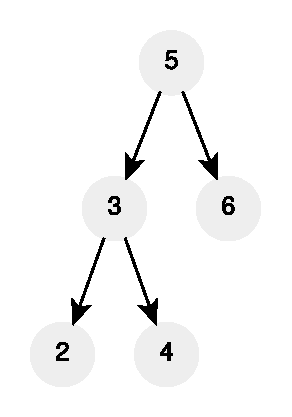
\includegraphics[width=\textwidth]{sources/merge_k_sorted_lists/images/example1}
%   \caption[Sample short cpation]{Sample Caption}.
%   \label{fig:merge_k_sorted_lists:example1}
%\end{figure}

\chapter{Merge $k$ sorted lists}
\label{ch:merge_k_sorted_lists}
\section*{Introduction}
The problem discussed in this chapter is quite interesting because it is rooted in the familiar merge-sort algorithm\cite{wiki:mergesort} which is a divide and conquer algorithm that works by first splitting a list into smaller and smaller ones (see figure \ref{fig:merge_k_sorted_lists:example_mergesort}) and after each of them is individually and separately sorted it merges them a pair at the time preserving the sorting property (see figure \ref{fig:merge_k_sorted_lists:example_mergesort_1}). 
In this chapter, we will focus on only one of these phases, specifically the merge phase and, we will try to find an efficient way to augment it so that it will be capable of merging more than only a pair of sorted lists. 

Coming up with a brute-force solution for merging $k$ lists is not hard but the resulting end algorithm is rather inefficient. 
A faster and more efficient approach requires a bit more effort, and in the remainder of the chapter, we will investigate a couple of different approaches that we can take to solve this problem efficiently.
In particular, we will have a look at the brute-force solution (in Section \ref{merge_k_sorted_lists:sec:bruteforce}) and then in Section \ref{merge_k_sorted_lists:sec:priorityqueue} to an approach that allows us to lower the time complexity quite a bit.


\begin{figure}
    \centering
    \begin{subfigure}[t]{0.80\textwidth}
        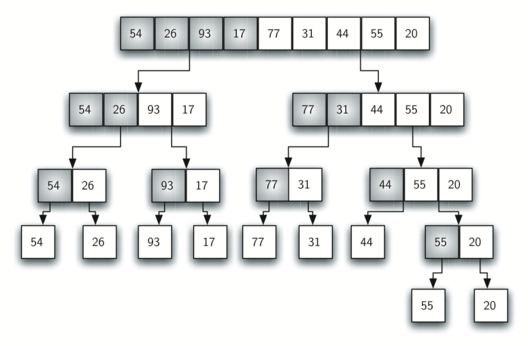
\includegraphics[width=\textwidth]{sources/merge_k_sorted_lists/images/mergesort_example}
        \caption[]{First phase of the merge-sort where the a list is recursively split into smaller ones (~ half the original length) until we are left with lists of size $1$}.
        \label{fig:merge_k_sorted_lists:example_mergesort}
     \end{subfigure}
    \hfill
    \begin{subfigure}[t]{0.80\textwidth}
        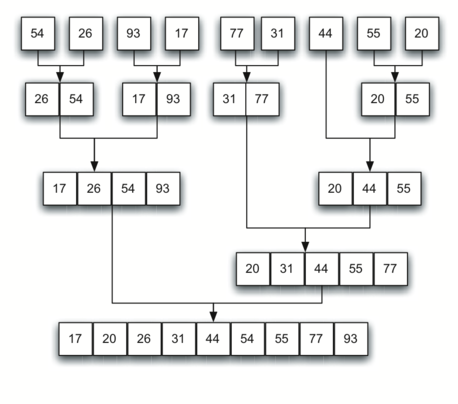
\includegraphics[width=\textwidth]{sources/merge_k_sorted_lists/images/mergesort_example_1}
        \caption[]{Second phase of the merge-sort where the split lists are recursively merged preserving the sorting property.}.
        \label{fig:merge_k_sorted_lists:example_mergesort_1}
     \end{subfigure}
\end{figure}

\section{Problem statement}
\begin{exercise}
\label{example:merge_k_sorted_lists:exercice1}
Write a function that, given $k$ lists that are sorted in ascending order, merges them into a new sorted list.

    %example1
    \begin{example}
        \label{example:merge_k_sorted_lists:example1}
        \hfill \\ 
        Given \inline{L=[[1,4,5],[1,3,4],[2,6]} the function returns \inline{[1,1,2,3,4,4,5,6]}
    \end{example}

    %example2
    \begin{example}
        \label{example:merge_k_sorted_lists:example2}
        \hfill \\ Given \inline{L=[[1,2,3],[4,5,6],[7,8,9]} the function returns \inline{[1,2,3,4,5,6,7,8,9]}
    \end{example}

    \begin{example}
        \hfill \\ Given \inline{L=[[7,8,9],[4,5,6],[1,2,3]} the function returns \inline{[1,2,3,4,5,6,7,8,9]}
    
    \label{ex:merge_k_sorted_lists:example3}
    \end{example}

\end{exercise}

%\section{Clarification Questions}
%\begin{QandA}
    %\item 
    %\begin{answered}
        %\textit{}
    %\end{answered}
    
%\end{QandA}

\section{Discussion}
\label{merge_k_sorted_lists:sec:discussion}


\subsection{Brute-force}
\label{merge_k_sorted_lists:sec:bruteforce}
There is clearly a naive way of approaching this problem which involves maintaining a master list (let's refer to it as \inline{sinkList}, which is initially empty), where the content of all $k$ lists will eventually end up, and merging the content of each individual list into it. 
Merging the \inline{sinkList} with the $i^{th}$ input list $L_i$ can be done exactly in the same way the merge sort does it. 
Repeating the process of merging the \inline{sinkList} with all the $k$ input lists eventually result in \inline{sinkList} being exactly what we need to return and will contain all the data in the $k$ input lists in the right order.

Listing \ref{list:merge_k_sorted_lists_bruteforce} shows an implementation of this idea.

\lstinputlisting[language=c++, caption={Brute-force solution reusing the two-list merging algorithm from the merge-sort algorithm.},label=list:merge_k_sorted_lists_bruteforce]{sources/merge_k_sorted_lists/merge_k_sorted_lists_solution1.cpp}

The code work by having a driver function \inline{merge_k_sorted_list_brute_force} issuing $k-1$ calls to another function called \inline{insert_sorted(Node <int >* sinkList , Node <int >* toBeInserted )}. The latter implements exactly what the merge phase of the merge sort does with the exception that it does so merging the nodes of its second parameter \inline{toBeInserted} directly into the first one \inline{sinkList} ( effectively dismantling \inline{toBeInserted} which would not be useable after the function returns).

The complexity of Listing \ref{list:merge_k_sorted_lists_bruteforce} is $O(n^2)$ where $n$ is the sum of the sizes of all input lists. The space complexity is $O(1)$ which is optimal as the returned list is constructed from the actual nodes that make up the $k$ input lists.


\subsection{Priority-queue approach}
\label{merge_k_sorted_lists:sec:priorityqueue}
We can do way better than quadratic time if we are clever in using a priority queue. 
What we will try to do here is to insert one node at a time into the \inline{sinkList}. 
At the beginning \inline{sinkList} is empty and the first node will surely be the smallest among all the first nodes of the $k$ input lists. Say list $i$ had the smallest element; we now remove it from list $i$ and add it to the \inline{sinkList}.
From where will the second node come from? Again it must be one (the smallest) of the first elements of the $k$ input lists! 
In other words, because the individual lists are sorted, the \quotes{next} element to be inserted in \inline{sinkList} must come from the front of the input lists.
Why not use a priority queue to keep track of the smallest element among all fronts of the input lists? If we do so, all it is necessary is to pick whatever node $n$ is at the top of the queue, insert it to the \inline{sinkList} and top up the queue a brand new node which will come from the same list $n$ belonged to.

The advantage of this approach is clear once we realize that now each element we get from the priority queue must be simply appended at the end of \inline{sinkList}. Appending at the end of a list is a simple operation that can be performed in constant time.
What about the price we pay for the priority queue? Both \inline{pop} and \inline{insert} operations have $log(k)$ time complexity (the priority queue will only contain the front element of each of input lists). Therefore the entire algorithm will have $nlog(k)$ and $O(k)$ time and space complexity respectively.

Listing \ref{list:merge_k_sorted_lists_prioqueue} shows an implementation of this idea.

\lstinputlisting[language=c++, caption={Priority-queue-based solution.},label=list:merge_k_sorted_lists_prioqueue]{sources/merge_k_sorted_lists/merge_k_sorted_lists_solution2.cpp}

The code works by first creating a \inline{std::priority_queue} having as underlying storage a \inline{std::vector} of \inline{NodeWrapper} which, as the name suggests, is a wrapper around a normal List \inline{Node} that also carries the information about the queue it belongs to.

The first loop of the function takes care of adding the first $k$ nodes in the queue.
The rest of the code is relatively straightforward with the main \inline{while} loop \inline{pop}ping the top element out of the queue (it is done by unpacking a \inline{NodeWrapper} into its components: \inline{ptr} and \inline{idx}, the pointer to the actual list's \inline{Node} and the index of the list this node belongs to) appends it at the end of the \inline{sinkList} and then proceeds in adding a new element into the queue that is drawn from the very same queue the last element popped out the queue belonged to (this info is stored in \inline{idx}). This element could of course not always exists when \inline{ptr} is the last element of the list number \inline{idx}.

When the queue is empty, we have finally inserted every element in the $k$ list and we can return \inline{sinkList} which now contains all the $n$ elements in all input lists in the proper order.

%\subsection{Divide et impera}
%\label{merge_k_sorted_lists:sec:divideetimpera}

